\section{Biologische Evolution}
\subsection{Vererbung und Verhalten}
\subsubsection{Verhaltensgenetik}
Wie hoch ist der Erblichkeitsanteil eines psychischen Phänomen?

Welche spezifischen Gene sind mit einem psychischen Phänomen assoziiert?

\begin{itemize}
	\item Genom-weite Assoziationsstudien: 
		\begin{itemize}
			\item Welche Gene sind mit einem psychischen Phänomen assoziiert?
			\item Korrelatives Studiendesign: Assoziationsstudien liefern nur Hinweise auf mögliche genetische Krankheitsfaktoren, keine genetische Ursachen!
			\item Die Einflüsse einzelner Gene auf Erleben und Verhalten sind meist minimal!
		\end{itemize}
	\item Anlage-Umwelt Interaktion:
		\begin{itemize}
			\item Wie interagieren Gene und Umwelt?
			\item Anlage-oder-Umwelt ist die falsche Frage: Beide
					wechselwirken, d.h. Interaktion!
		\end{itemize}
\end{itemize}
\subsection{Gehirn und Verhalten: Makro-Struktur und Funktion}
\subsubsection{Struktur des menschlichen Nervensystems}
\begin{center}
\tikz\graph [tree layout, sibling distance=1cm, nodes={rectangle, draw}]{Nervensystem--{Zentralnervensystem, Peripheres Nervensystem -- {Somatisches Nervensystem, Autonomes Nervensystem -- {Sympatikus, Parasympatikus}}}};
\end{center}
\begin{itemize}
	\item Zentralnervensystem
		\begin{itemize}
			\item Gehirn und Rückenmark
		\end{itemize}
	\item Peripheres Nervensystem
		\begin{itemize}
			\item neuronales Gewebe außerhalbvon Gehirn und Rückenmark
		\end{itemize}
	\item Somatisches Nervensystem
		\begin{itemize}
			\item sensorische und motorische Nerven, willkürlich
		\end{itemize}
	\item Autonomes Nervensystem
		\begin{itemize}
			\item internes System, nicht willkürlich
		\end{itemize}
	\item Sympatikus
		\begin{itemize}
			\item Notfall
		\end{itemize}
	\item Parasympatikus
		\begin{itemize}
			\item Wartung
		\end{itemize}
\end{itemize}
\subsubsection{Makro-Struktur des Gehirns}
\begin{center}
	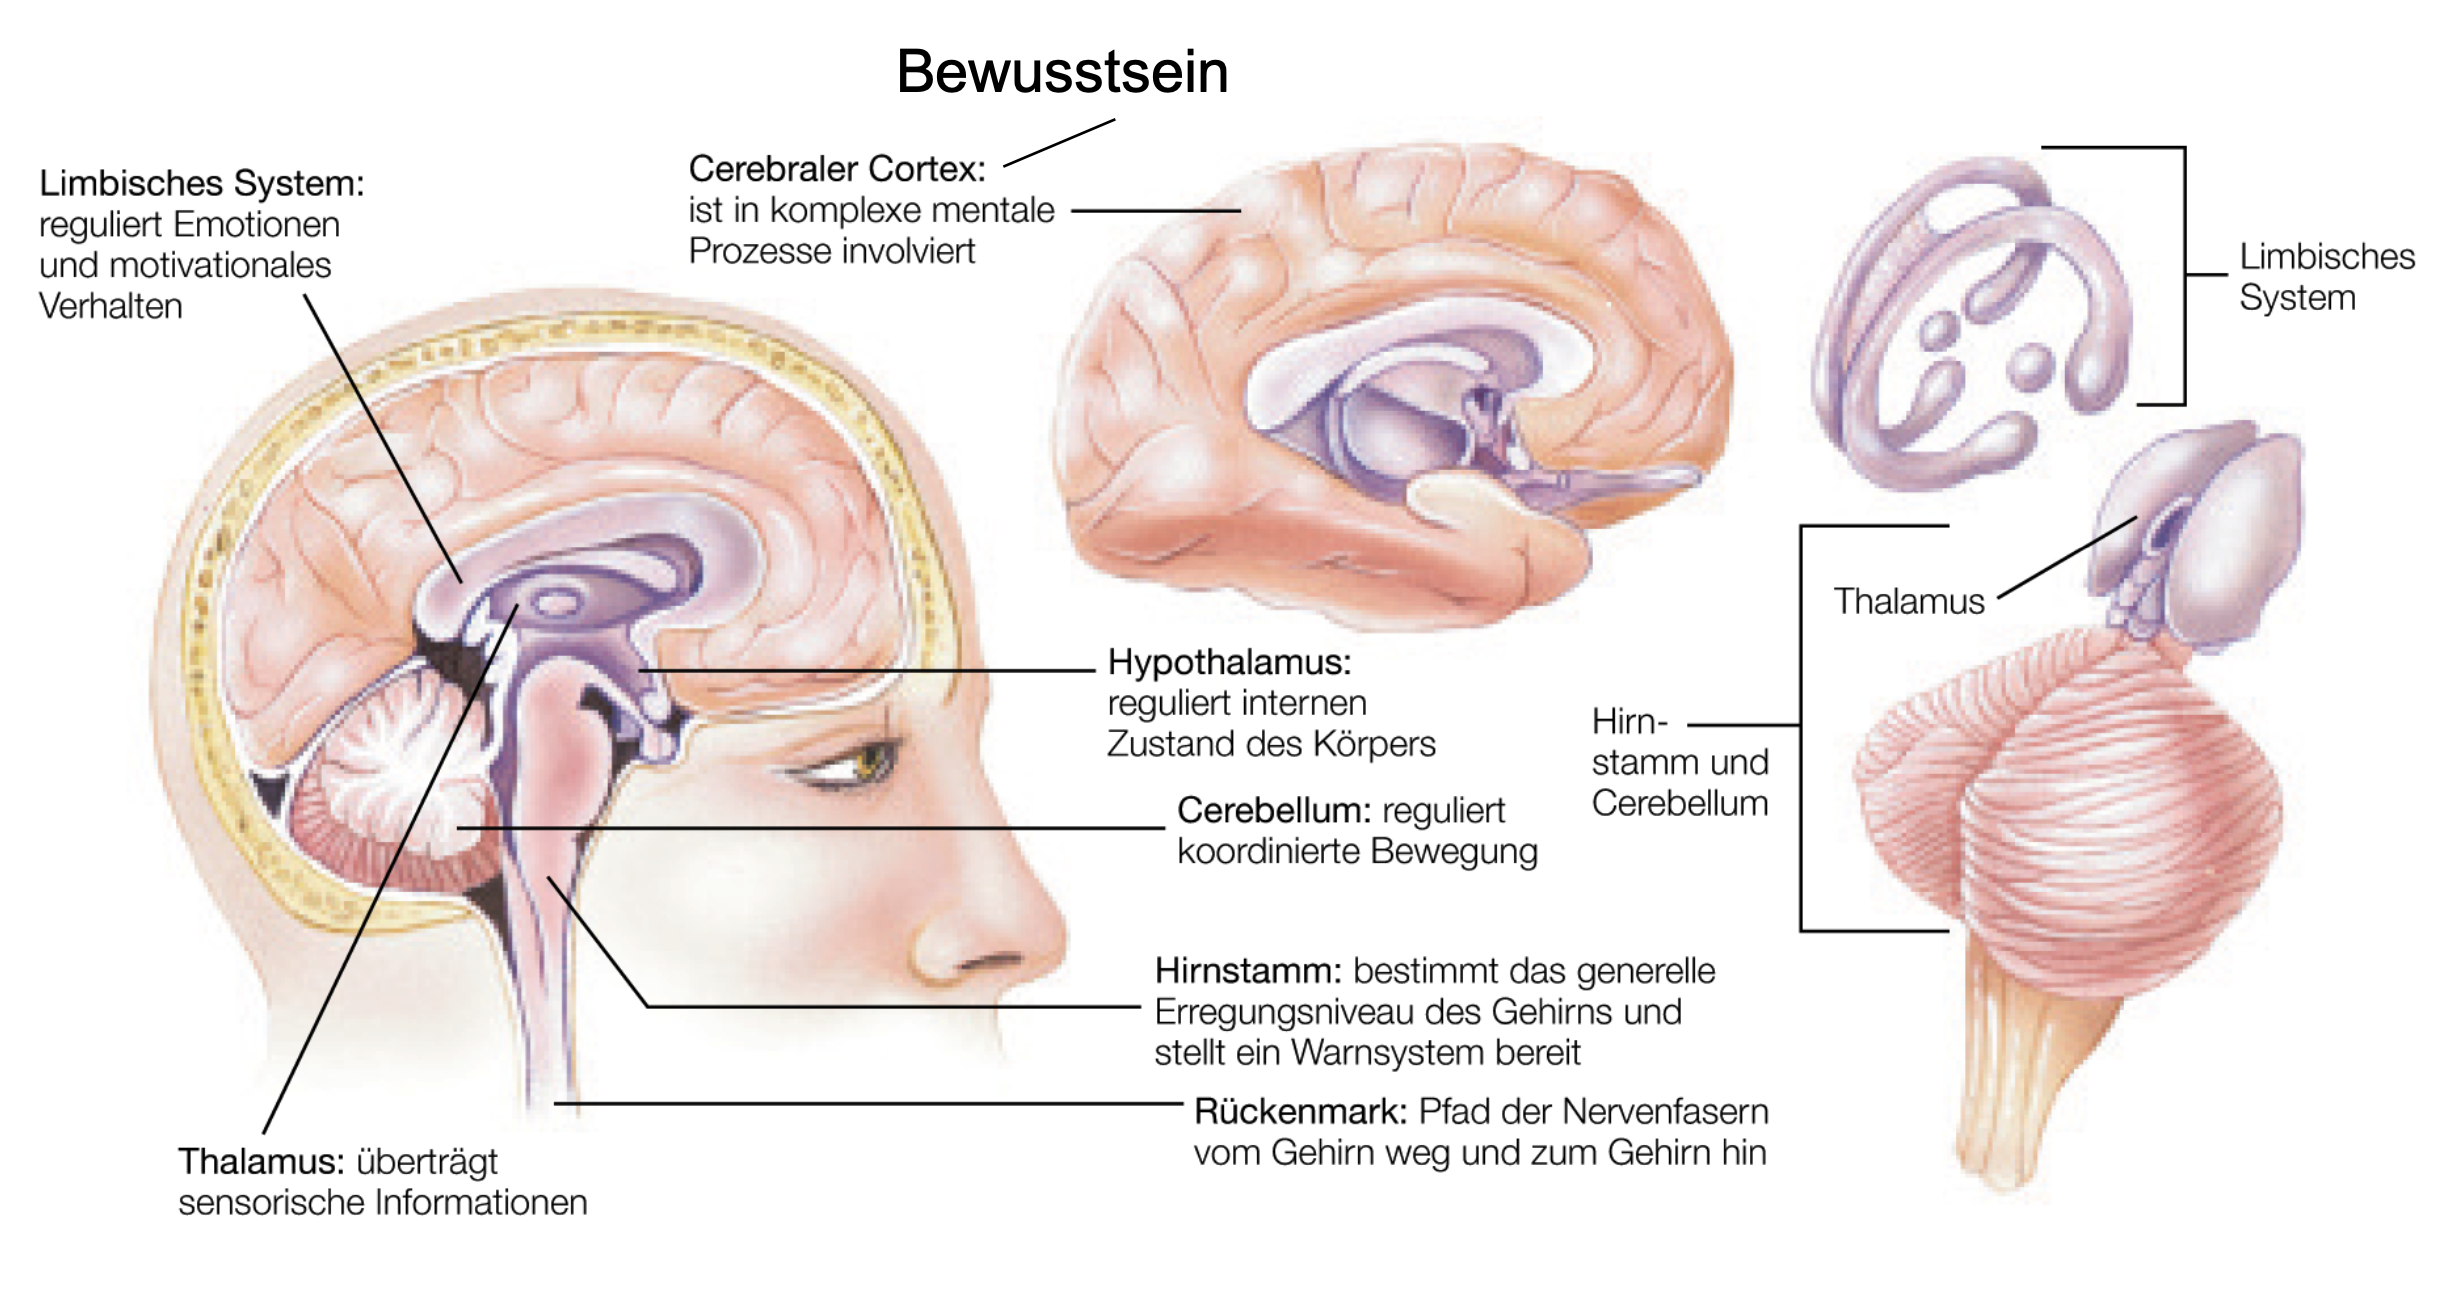
\includegraphics[scale=.25]{img/Gehirn.png}
\end{center}
\subsubsection{Hemisphärenlateralisation}
\begin{itemize}
	\item Linke Hemisphäre: Sprachlich-analytische
			sequentielle Fähigkeiten
	\item Rechte Hemisphäre: ganzheitlich-kreative
			parallele Fähigkeiten
	\item Nur relative
			Dominanz einer Hemisphäre, keine
			absolute!
\end{itemize}
\subsection{Gehirn und Verhalten: Mikro-Struktur und Funktion}
\subsubsection{Synaptische Übertragung}
Synaptische Übertragung durch Neurotransmitter und „Verrechnung“ im Soma des nachfolgenden Neurons

Wichtigste Neurotransmitter:
\begin{itemize}
	\item Glutamat (erregend)
	\item Gamma-amino-Buttersäure (GABA, hemmend)
	\item Dopamin
	\item Noradrenalin
	\item Serotonin
	\item Acetylcholin
	\item Endorphine
\end{itemize}

\subsubsection{Neuronale Plastizität}
Gehirnkapazität, die nicht genutzt wird atrophiert

















